\documentclass[tikz,border=5pt]{standalone}
\usetikzlibrary{calc}
\begin{document}
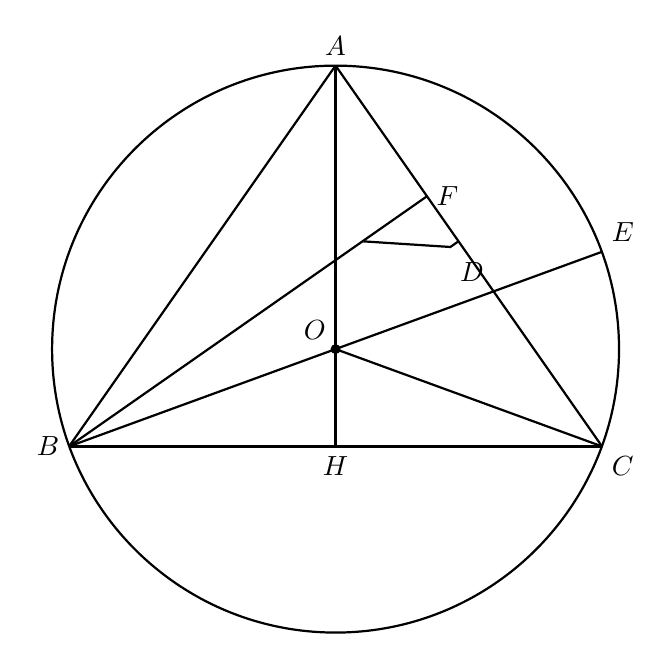
\begin{tikzpicture}[scale=1.2,>=stealth]
  % Circle and center
  \coordinate (O) at (0,0);
  \def\r{3}
  \draw[thick] (O) circle (\r);
  % Points
  \coordinate (A) at (0,3);
  \coordinate (B) at (-2.82,-1.03);
  \coordinate (C) at (2.82,-1.03);
  \coordinate (E) at (2.82,1.03);
  \coordinate (H) at (0,-1.03);
  % D = intersection of BE and AC
  \coordinate (D) at (1.672,0.611);
  % F = foot of perpendicular from B to AC
  \coordinate (F) at (0.967,1.617);
  % Solid lines
  \draw[thick] (A) -- (B);
  \draw[thick] (A) -- (C);
  \draw[thick] (B) -- (C);
  \draw[thick] (B) -- (E);
  \draw[thick] (B) -- (F);
  \draw[thick] (O) -- (C);
  \draw[thick] (O) -- (H);
  % AO now solid (formerly dashed)
  \draw[thick] (A) -- (O);
  % AH remains dashed
  \draw[thick,dashed] (A) -- (H);
  % Right angle at F
  \draw[thick] ($(F)!0.18!(C)$) -- ($($(F)!0.18!(C)$)!0.18!90:(F)$) -- ($(F)!0.18!(B)$);
  % Points
  \fill (O) circle (1.5pt);
  % Labels
  \node[above] at (A) {$A$};
  \node[left] at (B) {$B$};
  \node[below right] at (C) {$C$};
  \node[above right] at (E) {$E$};
  \node[above left] at (D) {$D$};
  \node[above left] at (O) {$O$};
  \node[right] at (F) {$F$};
  \node[below] at (H) {$H$};
\end{tikzpicture}
\end{document}
